\documentclass[a4paper,english,12pt,bibliography=totoc]{scrreprt}

\usepackage[T1]{fontenc} %immer
\usepackage[utf8]{inputenc} %am
\usepackage{babel} %Anfang

\usepackage{enumitem} %Aufzählungen verändern

%Gleichungen verwenden
\usepackage{newtxtext}
\usepackage{amsmath}
\usepackage{amssymb}
\usepackage{mathptmx}
%\usepackage{txfonts}

\usepackage{listings}% code blocks
\usepackage[most]{tcolorbox}

%Querverweise
\usepackage{varioref} %immer
\usepackage{hyperref} %in dieser
\usepackage{cleveref} %Reihenfolge

\usepackage{booktabs} %schönere Tabellen
\usepackage{siunitx} %SI-Einheiten
\usepackage{tabularx} %Tabellen mit flexiblen Spalten	

\usepackage{graphicx} %Grafiken verwenden

\usepackage[backend=biber,style=numeric]{biblatex}
\addbibresource{main.bib} 

\usepackage{lipsum} %Blindtext
\usepackage{subcaption}
\usepackage{afterpage}
\usepackage[headsepline]{scrlayer-scrpage} %Paket für Kopfzeilen
\usepackage{afterpage}
\usepackage{float}
\automark[subsection]{section}

\pagestyle{scrheadings}
\ihead{} % oben links
\chead{\leftmark} % oben Mitte
\ohead{} % oben rechts
\cfoot{\pagemark} % unten Mitte
\automark[section]{section} % Modified line

% Zu volle hboxen korrigieren
\tolerance 1414
\hbadness 1414
\emergencystretch 1.5em
\hfuzz 0.3pt
\widowpenalty=10000
\vfuzz \hfuzz
\raggedbottom

%Informationen über das Dokument
\date{\today}


\begin{document}


\begin{titlepage}
	\centering
	
\includegraphics[width=0.8\textwidth]{logo_uulm_sw}
	
	\vspace{1cm}
	\LARGE Laboratory Module for Master Programs
	\Huge \textbf{Biophysics Lab Course}
	
	\vspace{1cm}
	\Large Experiment:

	\Huge \textbf{Ligand binding}
	
	\vspace{15mm}
	\Large Performed on 19.06.2024
	
	\vspace{5mm}
	\LARGE Group 8
	
	\vspace{1cm}
	\Large
	\begin{tabular}{rcl}
	\textbf{Haiyang Zhang} & and & \textbf{Nicolae Turcan}\\
	\href{mailto:student.1@uni-ulm.de}{haiyang.zhang@uni-ulm.de} & & \href{mailto:student.2@uni-ulm.de}{nicolae.turcan@uni-ulm.de}
	\end{tabular}
	
	\vspace{7mm}
	Supervisor: Lisa Kwapich
	
	\vfill
	\begin{tabular}{p{50mm}@{\hspace{5cm}}p{50mm}}
	\hrulefill & \hrulefill \\
	%\centering Haiyang Zhang  & \centering Nicolae Turcan
	\end{tabular}
	
	\vspace{5mm}
	\normalsize \raggedright
	We hereby confirm that we have elaborated the present work and have detailed knowledge of the entire contents.
\end{titlepage}



\tableofcontents
\chapter{Abstract}
In this experiment, we investigated the ligand binding characteristics of Human Serum Albumin (HSA) with 3-Hydroxyflavone (3-HF) using Förster Resonance Energy Transfer (FRET) and Stern-Volmer analysis at different pH levels (pH 3 and pH 7). The study involved spectral characterization, binding curve analysis, and quenching dynamics to understand the interaction mechanisms. The absorption and emission spectra were recorded to calculate the Förster radius and evaluate the spectral overlap integral. The Stern-Volmer plots were generated to determine the quenching constants, and binding curves were fitted to obtain the half-saturation constant  and the Hill coefficient . The results indicated significant pH-dependent variations in binding affinity and quenching efficiency, with higher binding affinity observed at pH 7 compared to pH 3. This study provides insights into the environmental factors influencing HSA-3-HF interactions, contributing to the broader understanding of protein-ligand binding dynamics.
\label{cha:Abstract}

\chapter{Introduction}
\label{cha:Introduction}
During the past 15 years there has been a remarkable growth in the use of fluorescence in the biological sciences. It is widely employed in biological imaging, medical diagnostics, and materials science for its ability to selectively illuminate and detect specific molecules. The principle of fluorescence can be described using a Jablonski diagram (Figure 2.1). A fluorophore could reach the excited singlet state $S_1$ by photon absorption( $\mathrm{hV_A}$ ), then it may return to the ground state $S_0$ by photon emission ( $\mathrm{hV_F}$ ))and Radiative Decays ($\Gamma$ ) and Non-Radiative Decays ( k ) of which FRET is one of the possible decay pathways. 
\begin{figure}[H]
        \centering
        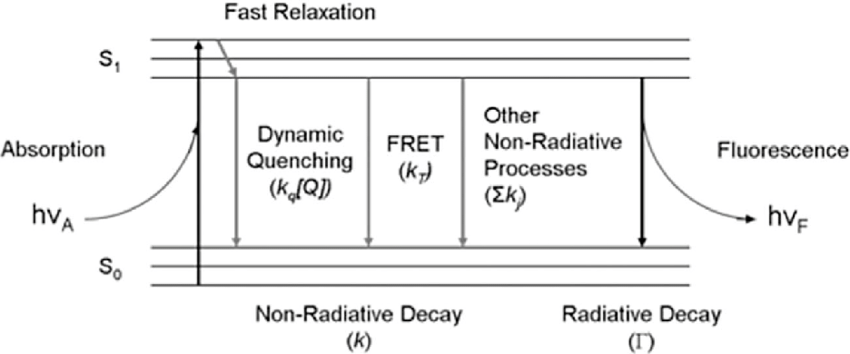
\includegraphics[width=0.9\textwidth]{Figures/A-simplified-Jablonski-diagram-illustrating-the-fluorescence-process-Photons-that-are(1).png}
	    \caption{Steric and energetic conditions for efficient Föster transfer}
\end{figure}

\[
\mathrm{Fluorescence}: S_1 \stackrel{k_F}{\longrightarrow} S_0 + h\nu_F
\]
\[
\mathrm{Nonradiative}: S_1 \stackrel{k_{nr}}{\longrightarrow} S_0
\]
Here $k_F$ and $k_{nr}$ are rate constants. For a system of N molecules at excited state $S_1$, the depopulation of the excited state is described by the following differential equation:
\[
\frac{dN}{dt} = -k_F\cdot N - k_{nr}\cdot N
\]
with the solution of the equation
\[
N(t) = N(0)exp(\frac{-t}{\tau_F})
\]
Where the lifetime of excited state(also called fluorescence lifetime) $\tau_F$ is given by the inverse sum of all rate coefficients:
\[
\tau_F = \frac{1}{k_F+k_{nr}}
\]

The fluorescence quantum yield is the number of emitted photons over the number of absorbed photons, which equal to the ratio of fluorescent transitions over all possible deactivation processes. It could be written in the ratio of rate coefficients of the corresponding process:
\[
\phi_f = \frac{k_f}{k_f+k_{nr}}
\]

This highlights that both radiative and non-radiative processes affect the fluorescence lifetime. Typically, fluorescence lifetimes span from picoseconds to nanoseconds, with around 10 nanoseconds being common.


However, in the real reaction process, solvent molecules and the chemical environment will interact with the excited fluorophores and lead to energy changes. The reversible reduction of fluorescence due to an additional nonradiative process caused by interaction with a second molecule is called quenching. \\

The fluorescence quenching can be categorized into two types, dynamic quenching and static quenching. In dynamic quenching, the excited fluorophores collide with a quencher molecule and return to the ground state nonradiatively. This leads to a reduction in the fluorescence lifetime and fluorescence quantum yield, which is shown in the formulas below.
\[
\tau = \frac{1}{k_F+k_{nr}+k_Q[Q]} \qquad \qquad   \phi = \frac{k_F}{k_F+k_{nr}+k_Q[Q]}
\]
which depends on the quencher concentration [Q], and $k_Q$ is the quenching rate coefficient. The ratios of unquenched and quenched lifetime and quantum yields are given by :

\[
\frac{\tau_0}{\tau} = \frac{\phi_0}{\phi} =  1 + \tau_0k_Q[Q] = 1+ K_{sv}[Q]
\]
where $K_{sv}$ is the Stern-Volmer constant, which describes the concentration dependence of quenching.\\

In static quenching, fluorophores are captured in nonfluorescent complexes and become two species of fluorophores: nonfluorescent fluorophore/quencher complexes and free fluorophores with unaffected fluorescence. In this case, the fluorescence signal will decrease but the fluorescence lifetime will not change, because only free fluorophores will contribute to the lifetime measurement.\\

A special case of fluorescence quenching is Föster resonance energy transfer(FRET), the nonradiative energy transfer from an excited molecule(donor) to another fluorophore(acceptor) by dipole-dipole coupling. \\

There are several requirements that need to be fulfilled for FRET. First, the donor and acceptor fluorophores have to be in close proximity, which in general, is less than 10 nm. Additionally, the donor and acceptor dipole orientations must be approximately parallel. Furthermore, the emission spectrum of the donor has to overlap with the absorption spectrum of the acceptor, as is shown in figure 2.2. And the distance dependence of the rate coefficient for energy transfer is found to be:
\[
k_{FRET}(R) = \frac{1}{\tau_D}(\frac{R_0}{R})^6
\]
and
\[
R_0 = (\frac{9ln(10)\kappa^2\phi_DJ}{128\pi^5N_An^4})^{1/6}
\]
\\
Here $k_{FRET}$ is the rate coefficient of FRET, and $R_0$ is called Förster radius, which characterizes the FRET pair. The $\phi_D$ is the fluorescence quantum yield of the donor, n is the refractive index, $\kappa^2$ is the orientation factor, and J is the overlap integral, which is:
\[
J = \int \epsilon_A(\lambda)f_D(\lambda){\lambda}^4\, d\lambda
\]

\begin{figure}[H]
        \centering
        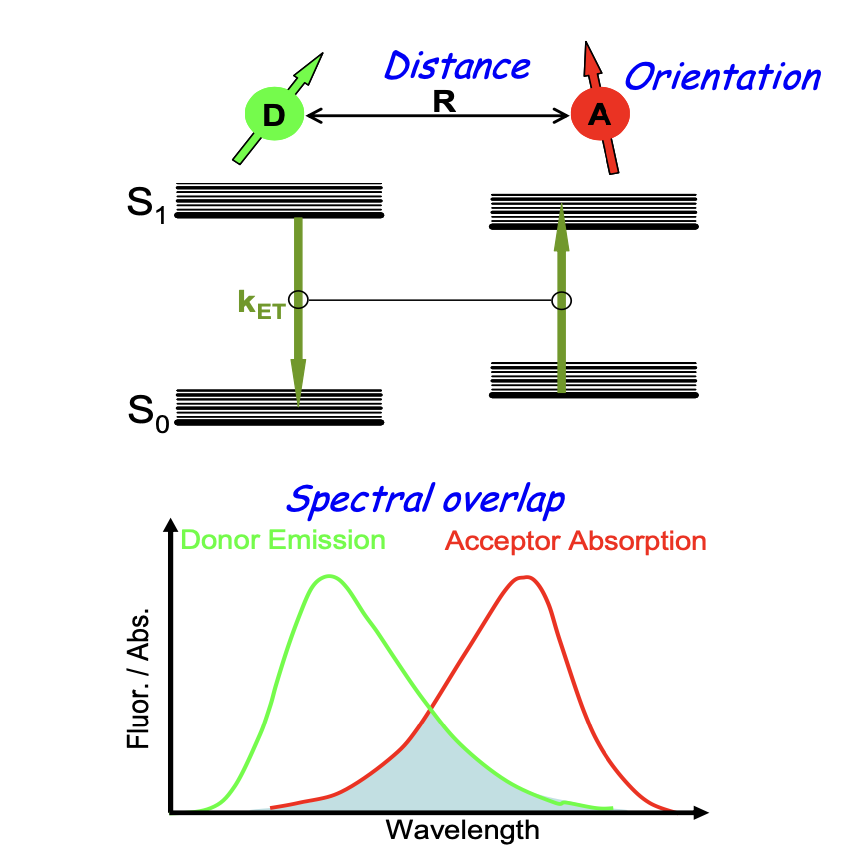
\includegraphics[width=0.8\textwidth]{Figures/FRET.png}
	    \caption{Steric and energetic conditions for efficient Föster transfer\cite{smFRET_lab_script}}
\end{figure}


Analyzing the relationship between quantum yield and fluorescence lifetime can reveal valuable information about the fluorophore's environment. For instance, lower quantum yield or shorter fluorescence lifetime might indicate increased non-radiative interactions or changes in the local environment.

In practical applications, these properties are often measured using time-resolved fluorescence spectroscopy, which involves exciting the fluorophore with a brief light pulse and observing the decay in fluorescence intensity over time. By fitting the decay to an exponential model, the fluorescence lifetime can be derived.

Quenching is the process that results in reduced fluorescence intensity of a fluorophore due to interactions with other molecules, known as quenchers. The main quenching mechanisms include dynamic (collisional) quenching and static quenching.

Dynamic quenching occurs when a fluorophore in its excited state collides with a quencher, causing non-radiative energy transfer and thus reducing fluorescence. This process is described by the Stern-Volmer equation:

\[
\frac{I_0}{I} = 1 + K_{SV}[Q]
\]

where $I_0$ is the initial fluorescence intensity, $I$ is the intensity in the presence of the quencher, $K_{SV}$ is the Stern-Volmer quenching constant, and $[Q]$ is the quencher concentration. This equation helps quantify the quenching efficiency.

Static quenching involves the formation of a non-fluorescent complex between the fluorophore and the quencher, reducing the number of excitable fluorophores. Unlike dynamic quenching, it does not depend on the excited state lifetime and varies with temperature and viscosity.

In some instances, both dynamic and static quenching can occur together, which can be analyzed using a modified Stern-Volmer equation:

\[
\frac{I_0}{I} = (1 + K_d[Q])(1 + K_s[Q])
\]

where $K_d$ and $K_s$ are the constants for dynamic and static quenching, respectively.

Understanding quenching mechanisms is essential for interpreting fluorescence data and is applied in fluorescence quenching assays to study molecular interactions, binding affinities, and conformational changes.


The theoretical background discussed so far applies only to dye pairs with a fixed spatial arrangement, resulting in a constant FRET efficiency for each dye pair. However, this experiment involves an ensemble measurement, which assumes that the two dyes are located on different molecules that can either bind or remain unbound, leading to a varied ensemble of molecules .

In this scenario, some donor molecules bind to acceptor molecules in close proximity, displaying a maximal FRET efficiency (\(E_{max}\)) determined by the binding geometry. The remaining donor molecules, which are unbound, exhibit a FRET efficiency of zero. Therefore, the average FRET efficiency (\(<E>\)) of the ensemble depends on the proportion of donor molecules that are in the bound state relative to the total concentration of molecules in the sample :

\[
<E> = E_{max} \cdot \frac{[DA]}{[D]_{tot}} + 0 \cdot \frac{[D]}{[D]_{tot}}
\]

where

\[
[D]_{tot} = [D] + [DA]
\]

The binding equilibrium is described by the law of mass action:

\[
\frac{1}{K_D} = \frac{[DA]}{[D]_{tot} + [A]}
\]

where \(K_D\) is the dissociation equilibrium constant. Thus, the experimentally measurable mean FRET efficiency relates to the free acceptor concentration as:

\[
<E> = \frac{E_{max}}{1 + \frac{K_D}{[A]}}
\]

By plotting the average FRET efficiency against the (logarithmic) acceptor concentration, one can infer both the spatial arrangement of the donor-acceptor pair (from the saturation value \(E_{max}\)) and the binding balance (from the half-saturation concentration \(K_D\)) .

In cases of cooperative binding, a Hill coefficient (\(n\)) must be considered, resulting in:

\[
<E> = \frac{E_{max}}{1 + \left(\frac{K_D}{[A]}\right)^n}
\]

which produces a binding curve with a steeper slope for \(n > 1\) .

In this experiment, the emission spectrum, including both donor and acceptor emission, is recorded at varying acceptor concentrations while the donor is excited. The transfer efficiency is then calculated from the fluorescence intensities of the respective emission peaks .

The transfer efficiency can be computed in different ways. One method involves calculating the transfer efficiency from the fluorescence quenching of the donor:

\[
E = \frac{I_D^0 - I_D}{I_D^0}
\]

where \(I_D\) and \(I_D^0\) are the measured donor intensities with and without the acceptor (quencher), respectively \cite{lab_script}.

Alternatively, the relation between the FRET-induced fluorescence of the acceptor (\(I_A\)) upon donor excitation and the transfer efficiency can be expressed as:

\[
E = \frac{I_A}{I_A + \gamma I_D}
\]

where \(\gamma\) is a correction factor that accounts for differences in the probabilities of excitation photon emission and detected emission photon between the donor and acceptor dyes \cite{FRET_}.

\chapter{Material and methods}
\section{Material}
\begin{table}[h]
\centering
\begin{tabular}{|>{\raggedright\arraybackslash}p{0.5\textwidth}|>{\raggedright\arraybackslash}p{0.4\textwidth}|}
\hline
\textbf{Materials} & \textbf{Details} \\
\hline
Solution A  & 10 mM sodium phosphate buffer (pH 7) 5 mg/ml HSA \\
\hline
Solution B  & 1 mM HCl solution (pH 3)  5 mg/ml HSA\\
\hline
Ligand Solution  & 1 mM 3-HF in ethanol 0.15 mg/ml  \\
\hline
\textit{Note: All solutions were provided by our instructor.} & \\
\hline
\end{tabular}

\vspace{1em}

\begin{tabular}{|>{\raggedright\arraybackslash}p{0.5\textwidth}|>{\raggedright\arraybackslash}p{0.4\textwidth}|}
\hline
\textbf{Equipment} & \textbf{Details} \\
\hline
Absorption spectrometer & Cary (see Fig. 3.1) \\
\hline
Fibre-coupled cooled CCD-spectrometer &  Model Ocean Optics QE Pro (see Fig. 3.2) \\
\hline
Fibre coupled LED source & Emission wavelength of 285 nm \\
\hline
Semi-micro cuvette & 4 × 10 mm \\
\hline
\end{tabular}
\end{table}

\begin{figure}[H]
    \centering
    \begin{subfigure}[b]{0.45\textwidth}
        \centering
        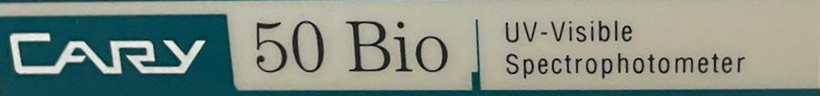
\includegraphics[width=\textwidth]{Instruments/Spectruophotometer.png} 
        \caption{hardware Model}
        \label{fig:subfigure1}
    \end{subfigure}
    \hfill
    \begin{subfigure}[b]{0.45\textwidth}
        \centering
        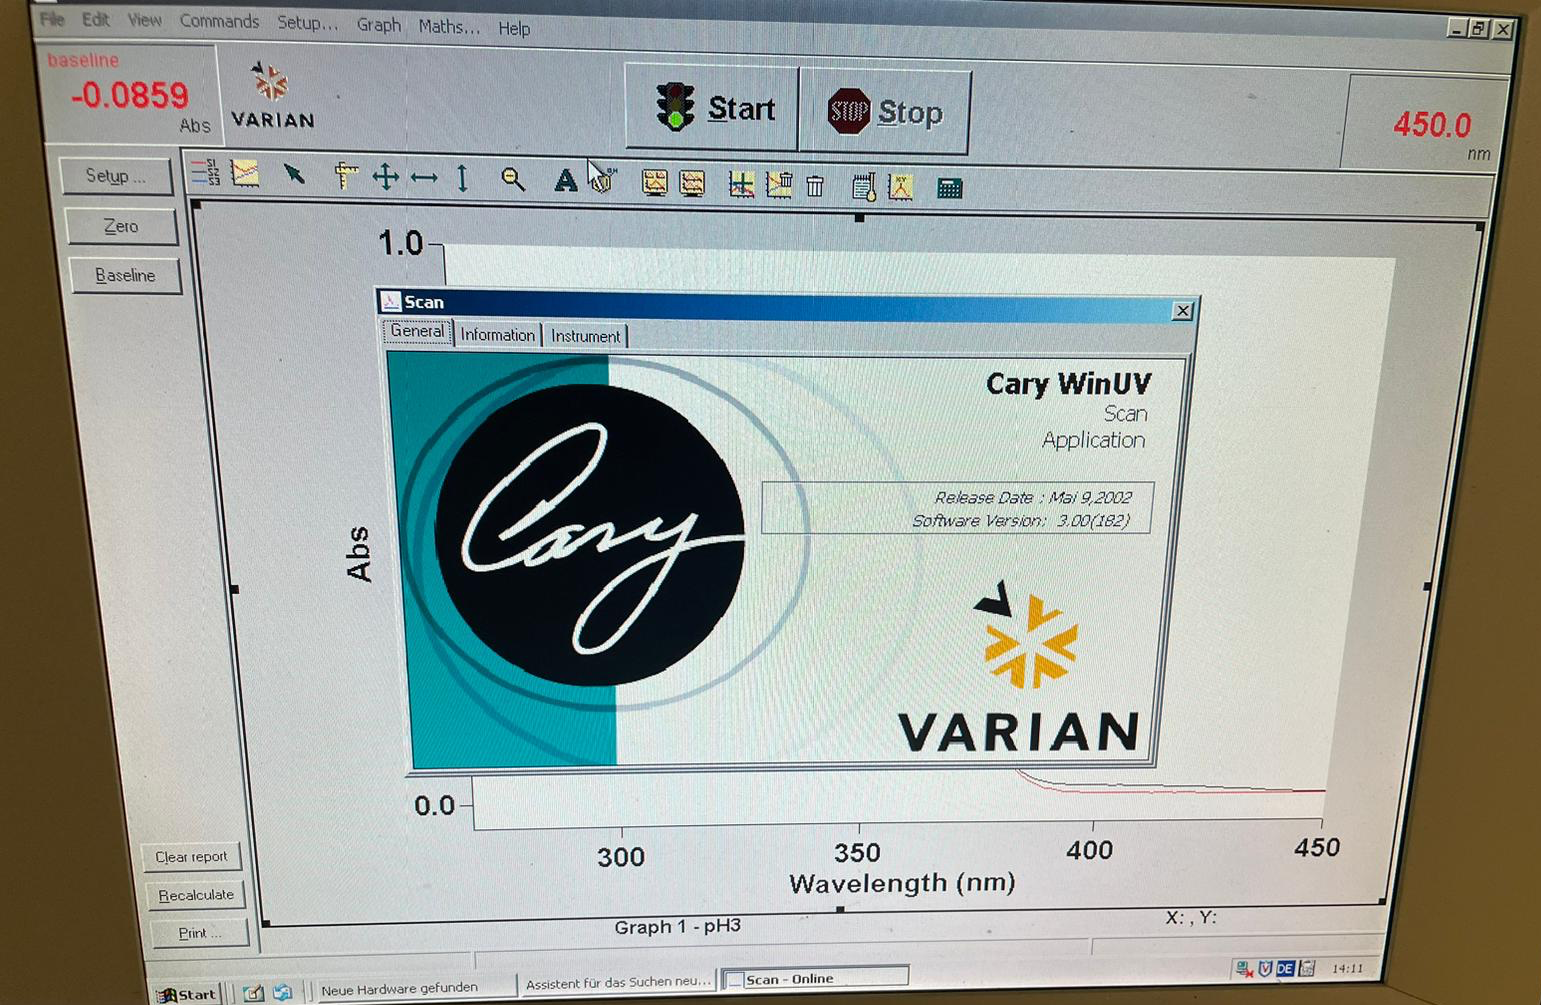
\includegraphics[width=\textwidth]{Instruments/software for absorption.png} % Replace with the path to your second image
        \caption{Software}
        \label{fig:subfigure2}
    \end{subfigure}
    \caption{Absorbance Spectrophotometer}
    \label{fig:mainfigure}
\end{figure}

\begin{figure}[H]
    \centering
    \begin{subfigure}[b]{0.45\textwidth}
        \centering
        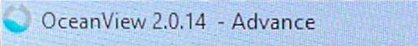
\includegraphics[width=\textwidth]{Instruments/emission software.png} % Replace with the path to your first image
        \caption{Software}
        \label{fig:subfigure1}
    \end{subfigure}
    \hfill
    \begin{subfigure}[b]{0.45\textwidth}
        \centering
        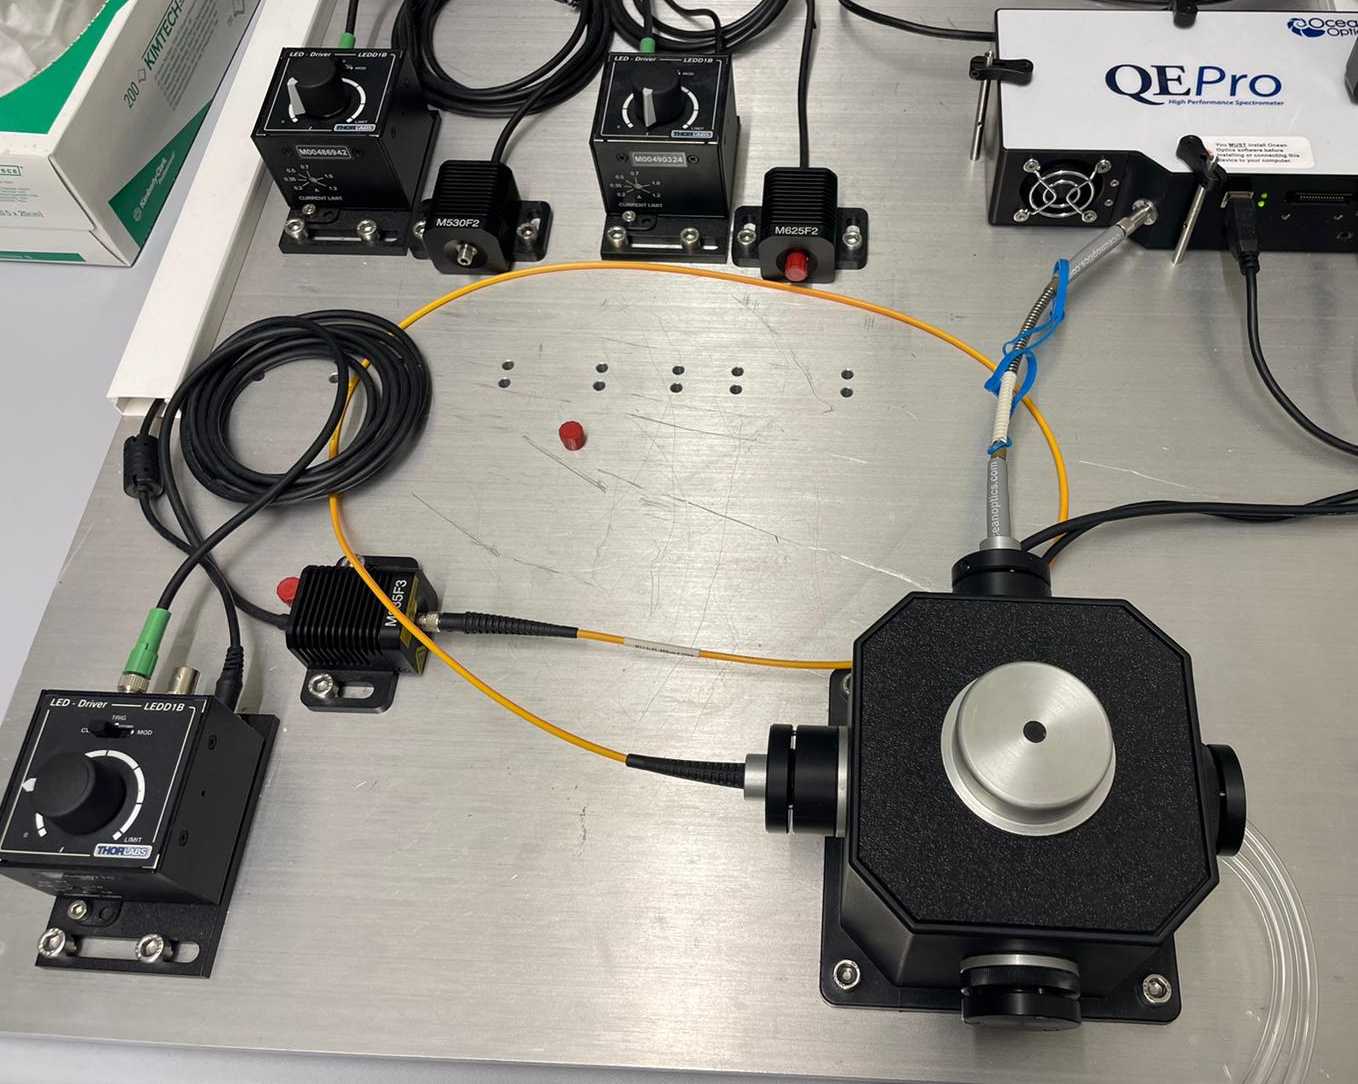
\includegraphics[width=\textwidth]{Instruments/spectrum meter.png} % Replace with the path to your second image
        \caption{Optical Setup of Instrument}
        \label{fig:subfigure2}
    \end{subfigure}
    \caption{Real Time Spectrophotometer}
    \label{fig:mainfigure}
\end{figure}

\section{Methods}

In this experiment, we used the following approximation to calculate the Förster radius. The overlap integral (\(J\)) is calculated using the approximation of an infinitely narrow emission spectrum of the donor, which means the peak of the emission spectrum of donor and acceptor are the same as the donor peak, and the overlap area is linear to the extinction coefficient, as is given in the following eqaution:

\begin{equation}
J = \epsilon_A(\lambda_D^{\text{Em}}) \lambda_D^{\text{Em}^4}
\end{equation}

The Förster radius was calculated using the following parameters:
\begin{itemize}
    \item Extinction coefficient of 3-HF: \(\epsilon_{345} = 10^4 \, \text{m}^{-1} \, \text{cm}^{-1}\)
    \item Refractive index: \(n = 1.4\)
    \item Quantum yield of Trp: \(\phi_D(\text{Trp}) = 0.11\)
    \item Orientation factor: \(\kappa^2 = \frac{2}{3}\) (Assuming free rotation)
\end{itemize}

By using the equation 3.2, we could calculate the Förster radius :
\begin{equation}
R_0 = \left( \frac{9 \ln(10) \kappa^2 \Phi_D J}{128 \pi^5 N_A n^4} \right)^{\frac{1}{6}}
\end{equation}



%Materials:The instruments used in experiment
%Methods: 
%1) The approximation method for determine the Foster distance.(Total overlap, same orientation, both maximum intensity equals to the intenisty of the emission spectrum.)
%2)FRET ensemble measurements, and how to use it to determine the %characteristics of the reaction (K_D, n, E_max)
\chapter{Experiment and results}
\label{cha:Experiment}

\section{Experiment}
During the experiment, we measured the absorption spectrum of 3-HF and a series of FRET emission spectra of the HSA-3-HF mixture. While measuring the absorption spectrum, 75 \textmu l of 3-HF was added into 1 ml of solution A (pH7) and solution B (pH3) and measured under an absorption spectrometer, with wavelength ranging from 270 nm to 450 nm. After that, we used the Fibre-coupled cooled CCD-spectrometer together with the optical instruments to measure the emission spectrum of the HSA and HSA-3-HF mixture. 40 \textmu l of HSA was added separately into 760 \textmu l of solutions A and B to measure the emission spectrum of HSA under different pH. Then for each group, we added 3-HF 15 times to the solution with the volume of 0.5, 0.5, 0.5, 0.5, 1, 1, 2, 2, 2, 5, 5, 10, 10, 20, 20 \textmu l and acquired a series of emission spectrum under different pH.

\begin{figure}[h]
    \centering
    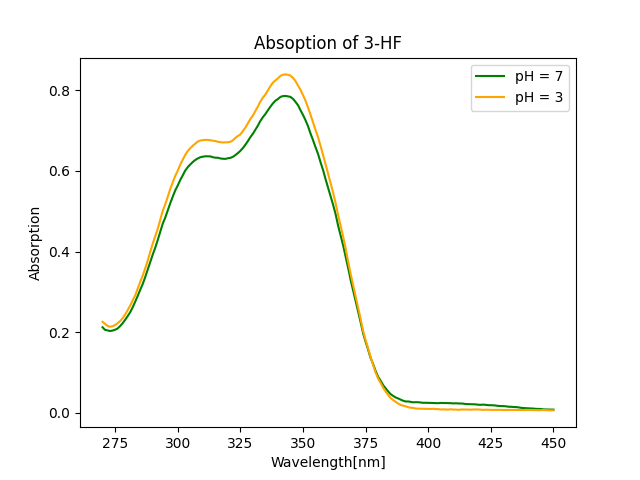
\includegraphics[width = 0.8\textwidth]{Figures/Absorption_3_HF.png}
    \caption{The absorption spectrum of the 3-HF under pH = 3 and pH = 7}
    \label{fig:enter-label}
\end{figure}
\section{Results}
% 1) absorption spectrum of the 3-HF

The absorption spectra of 3-HF under pH3 and pH7 are shown in Figure 4.1. \\

Figures 4.2 and 4.3 show the emission spectra of the HSA and 3-HF mixture changing over different 3-HF concentrations under different pH values. From the figure, we could clearly observe two peaks and the intensity change of the two peaks with respect to the acceptor (3-HF) concentration. By looking at the donor (HSA) emission spectrum (3-HF = 0), we could say that the left peak is the emission peak of the donor, while the right side peak is the acceptor emission peak. By analyzing the figures and data, we found the wavelength of the emission peaks is at 330nm (pH3) and 343nm (pH7).\\

\begin{figure}[h]
    \centering
    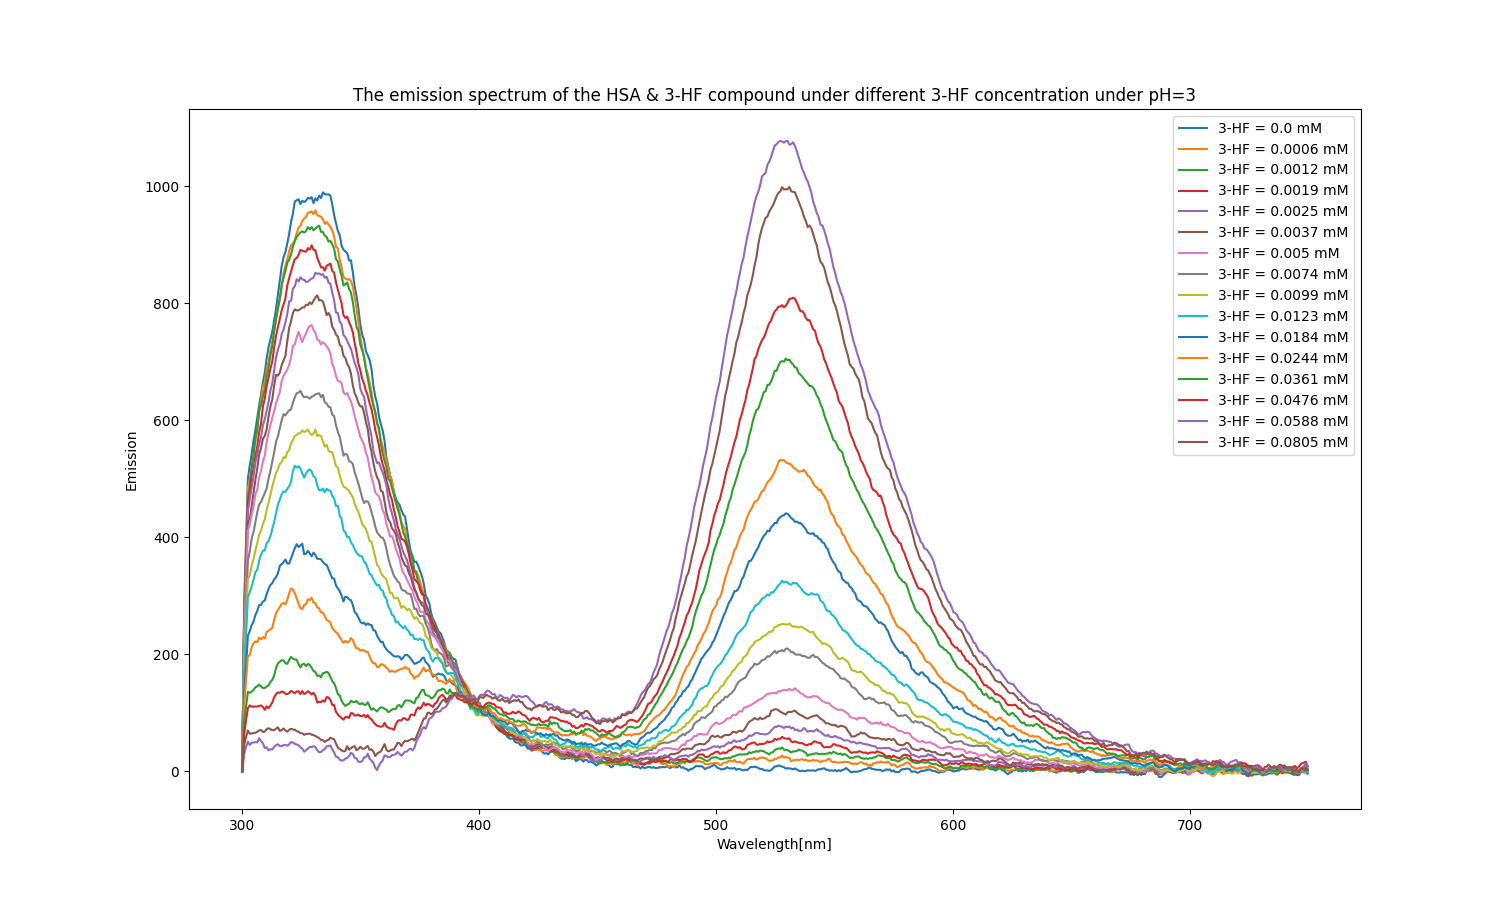
\includegraphics[width = 0.9\textwidth]{Figures/emission_ph3.png}
    \caption{The emission spectra of HSA and 3-HF under pH = 3 with changing 3-HF concentration}
    \label{fig:enter-label}
\end{figure}
\begin{figure}[h]
    \centering
    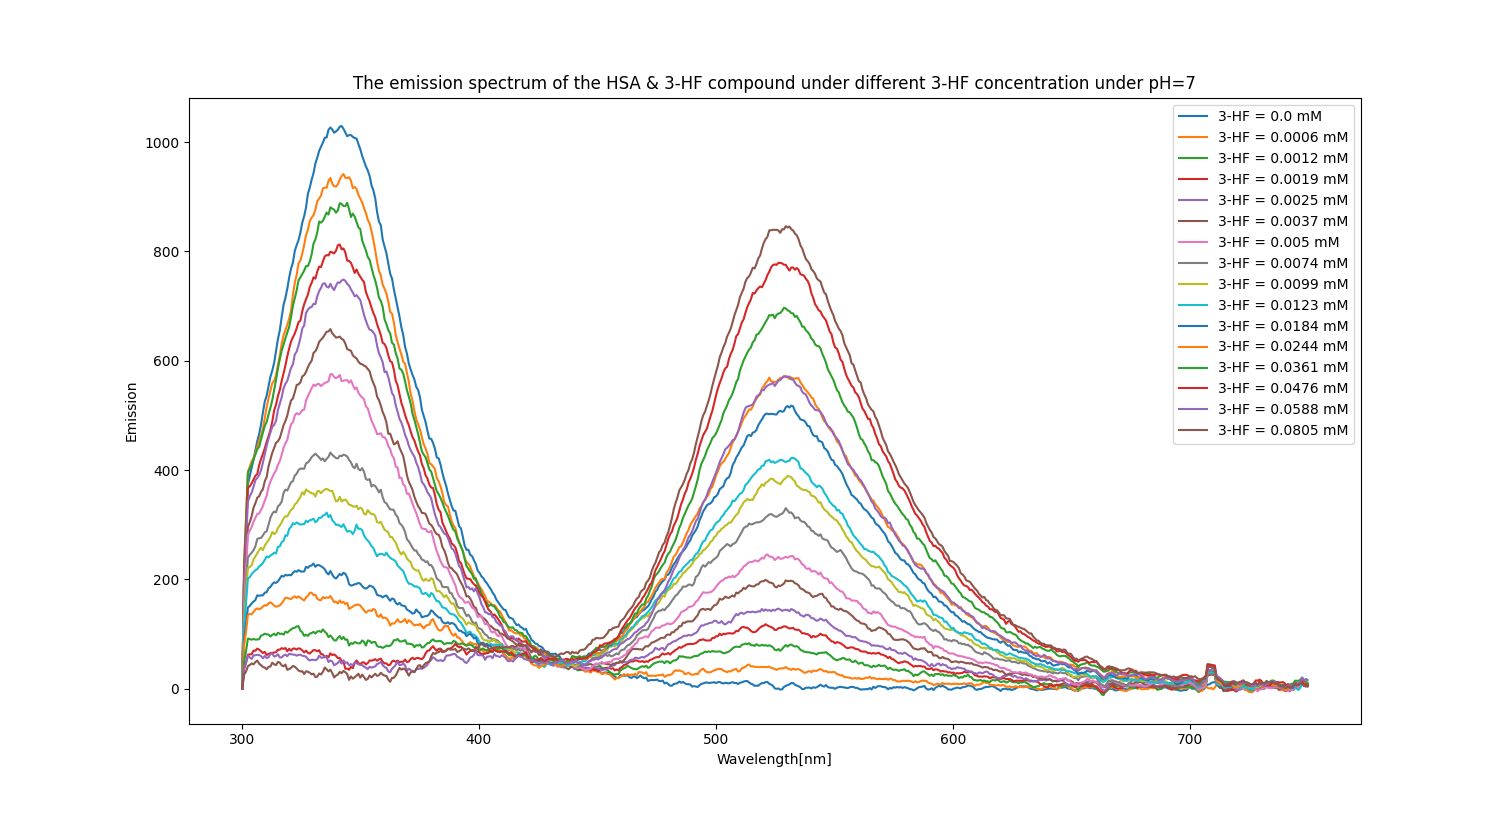
\includegraphics[width = 0.9\textwidth]{Figures/emission_ph7.png}
    \caption{The emission spectra of HSA and 3-HF under pH = 7 with changing 3-HF concentration}
    \label{fig:enter-label}
\end{figure}

After that, we did the Stern-Volmer plot (Figure 4.4). By setting the intercept to 1, we did the linear fitting of the concentration over $\frac{I_0}{I}$, thus the slope of the line is $K_{SV}$, which is 183.51/mM (pH3) and 294.30/mM (pH7). The $I_0$ was acquired at the emission peak of the donor while the concentration of the acceptor is 0. And $I$ represents the donor peak intensity depending on the concentration of 3-HF.\\

\begin{comment}
        E_max   K_D   n
ph3 1.06020631 0.01777591 1.42018972
ph7 1.09189907 0.01183027 1.00922149
(It's wired that the fitting results of E_max is larger than 1. That could because it's a fitting result...)
The emission maximum wavelength:
ph3: 329.542nm
ph7: 342.952nm
\end{comment}

% 2) The emission spectrum wrt the 3-HF concentration.

\begin{comment}
\begin{figure}[htbp]
    \centering
    \begin{subfigure}[b]{0.45\textwidth}
        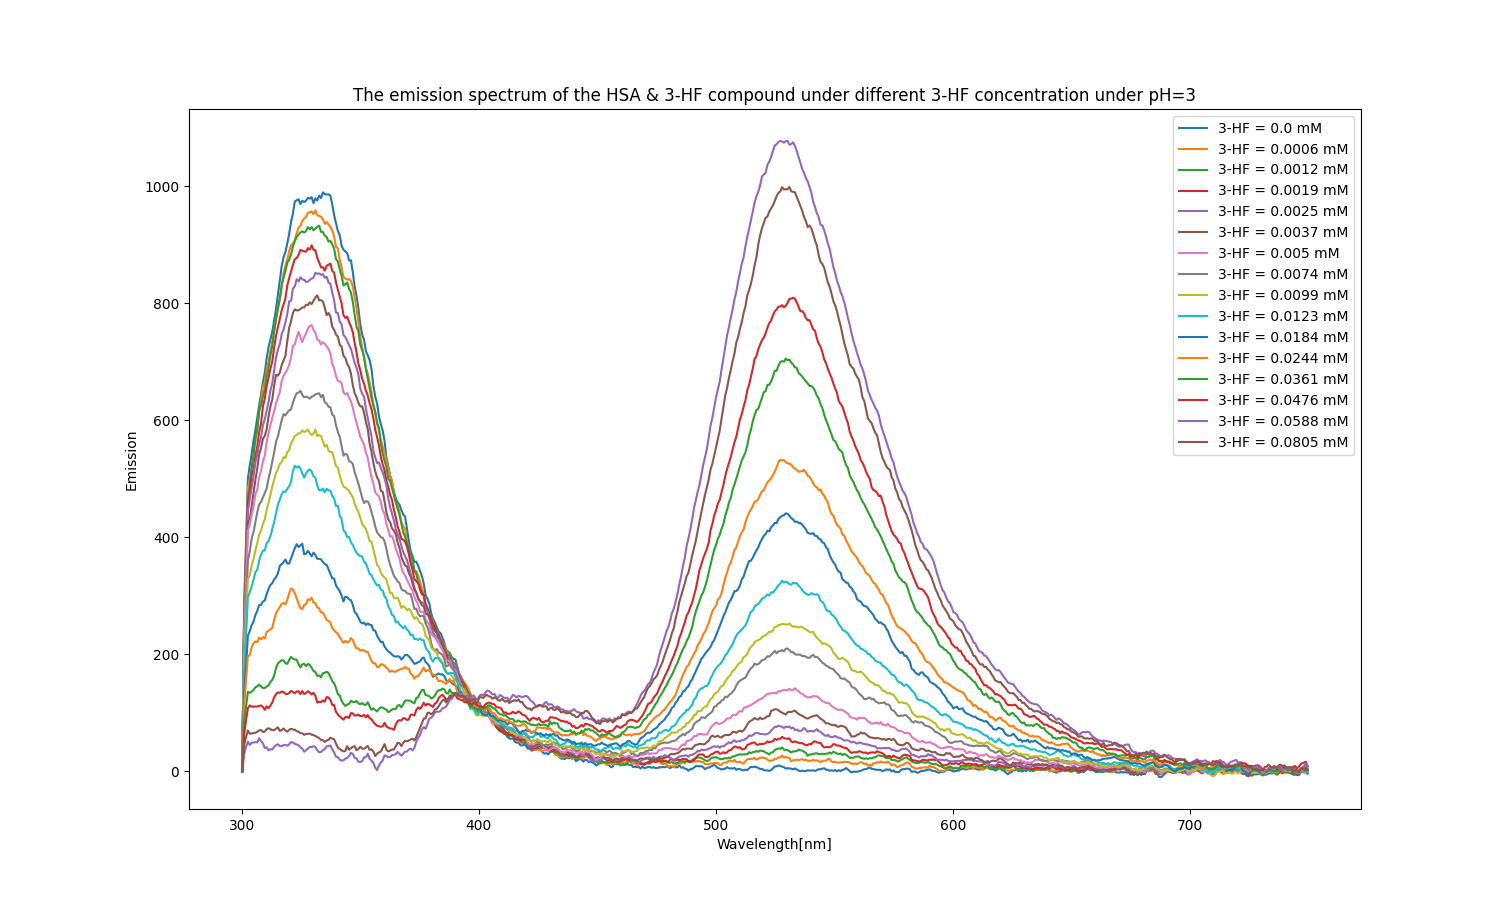
\includegraphics[width=\textwidth]{Figures/emission_ph3.png}
        \caption{ pH = 3}
    \end{subfigure}
    \quad % Adjust spacing between subfigures as needed
    \begin{subfigure}[b]{0.45\textwidth}
        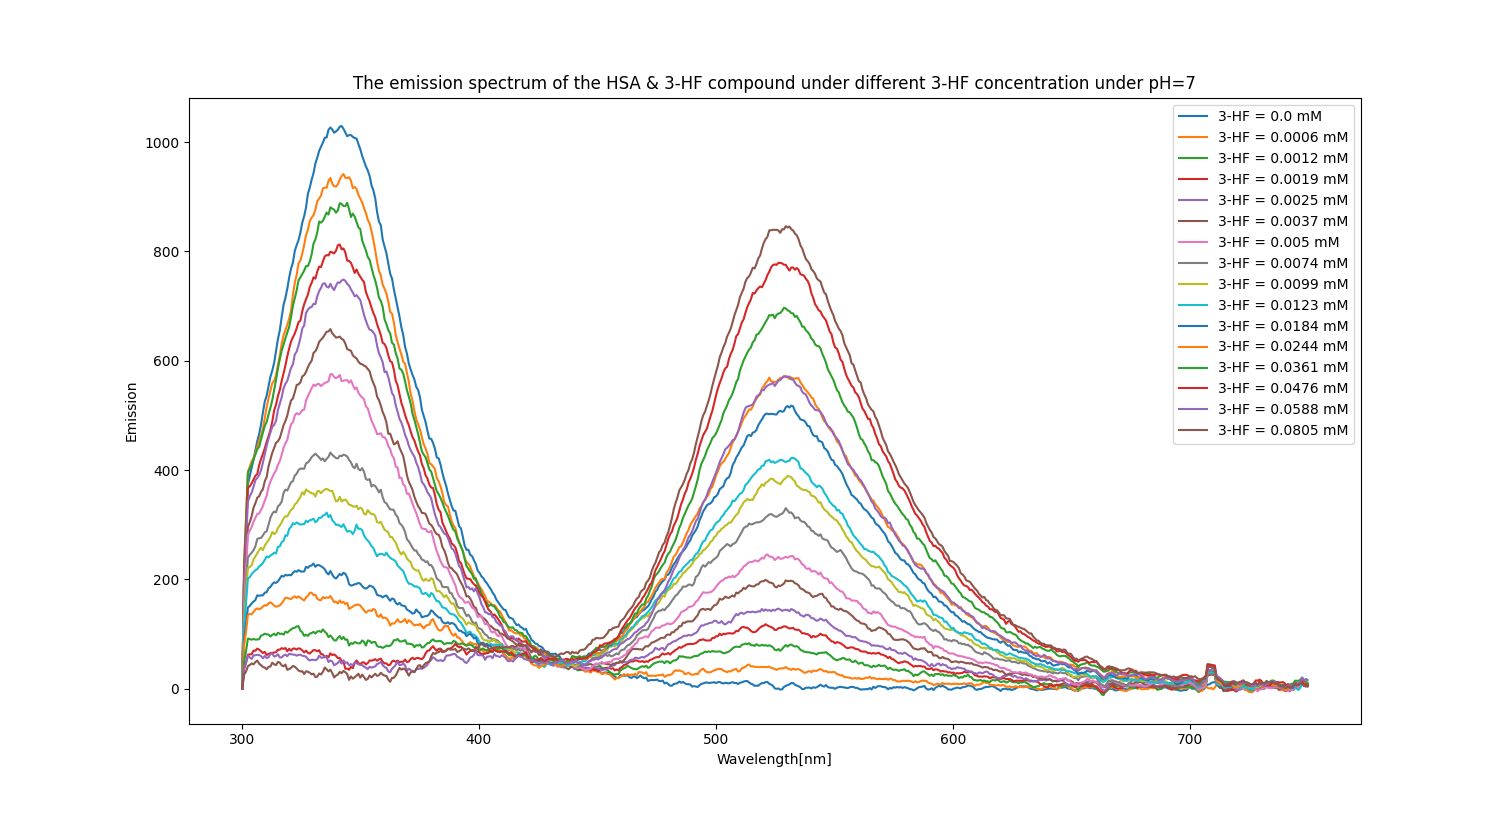
\includegraphics[width=\textwidth]{Figures/emission_ph7.png}
        \caption{pH = 7}
    \end{subfigure}
    \caption{The emission spectrum of HSA and FRET pair}
\end{figure}
\end{comment}


\begin{figure}[htbp]
    \centering
    \begin{subfigure}[b]{0.45\textwidth}
        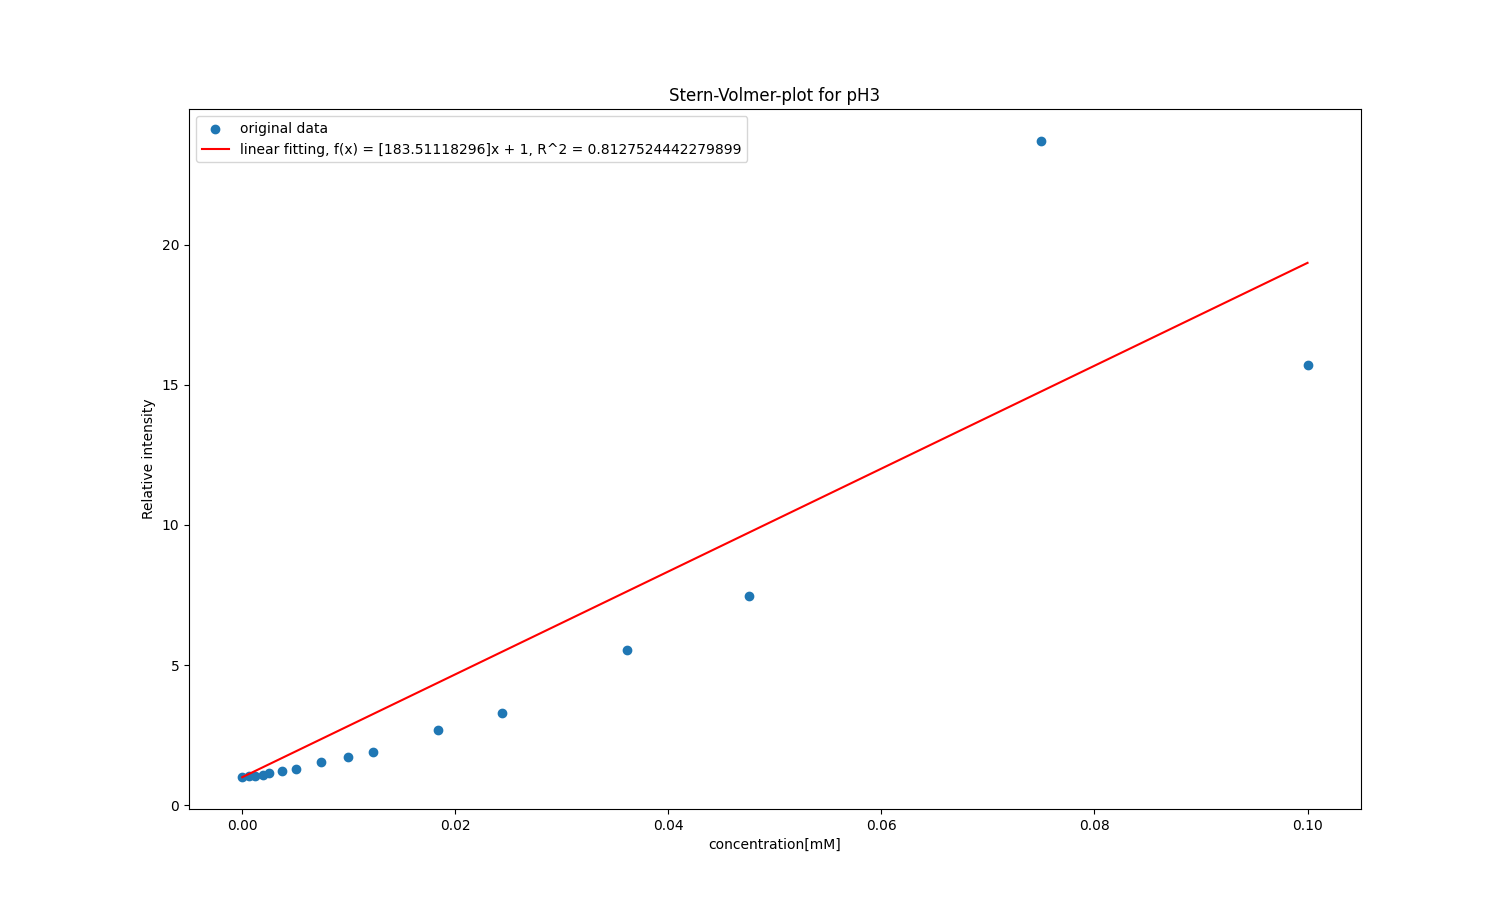
\includegraphics[width=\textwidth]{Figures/SV plot ph3.png}
        \caption{pH3}
    \end{subfigure}
    \quad % Adjust spacing between subfigures as needed
    \begin{subfigure}[b]{0.45\textwidth}
        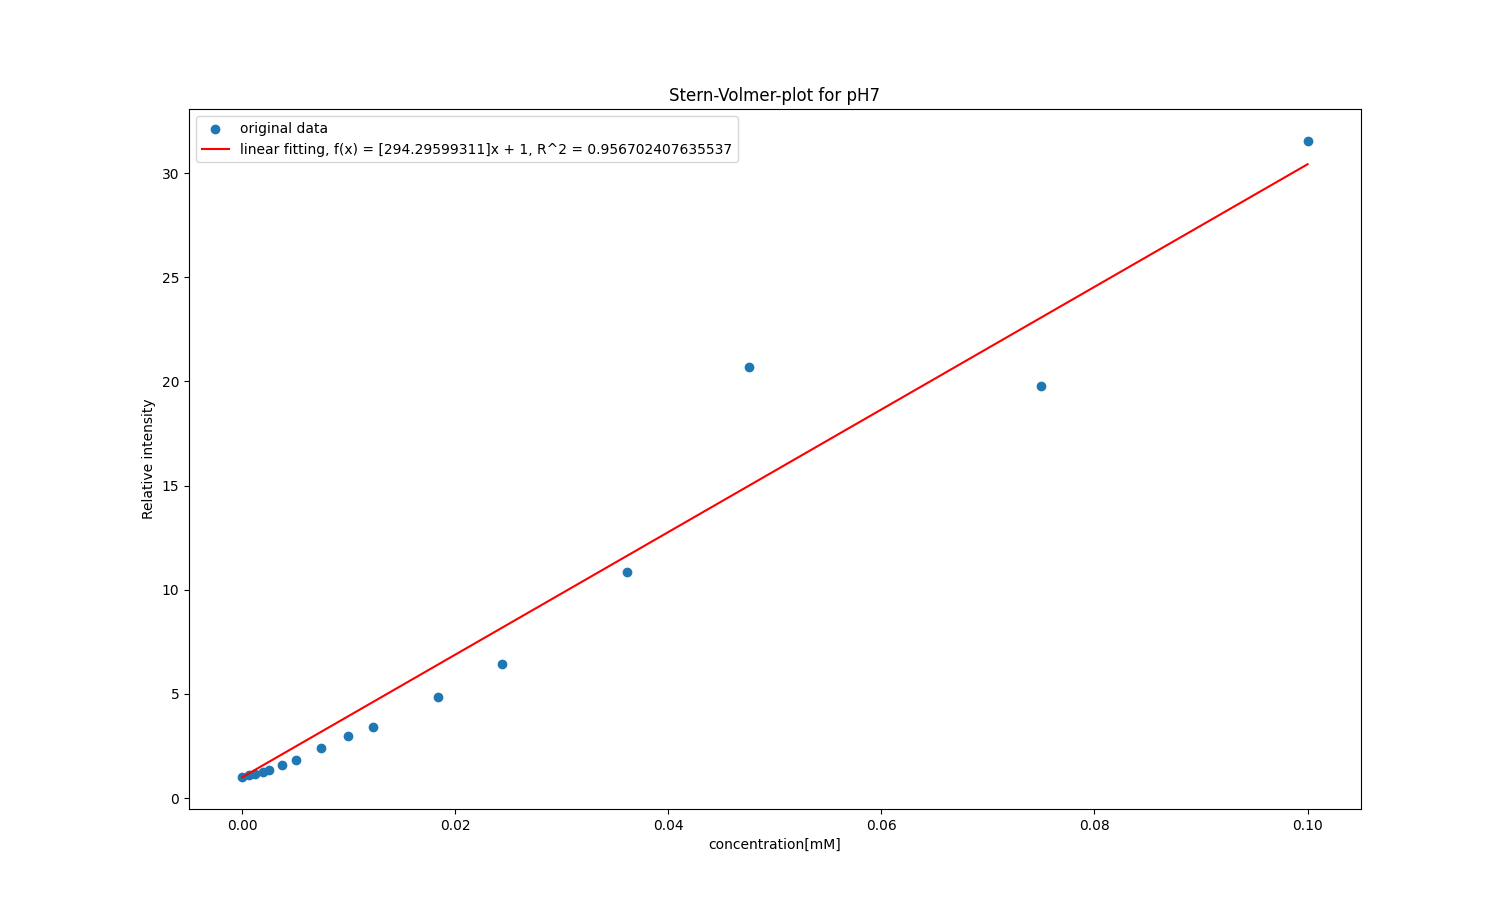
\includegraphics[width=\textwidth]{Figures/SV plot ph7.png}
        \caption{pH7}
    \end{subfigure}
    \caption{The Stern-Volmer plot}
\end{figure}

Further more, we calculated the ensemble FRET efficiency (<E>) using the emission intensity of donor and acceptor (see introduction, using $\gamma$ = 1 for pH3 and $\gamma$ = 0.7 for pH7) and plotted it over concentration of acceptor ([A], Figure 4.5 and 4.6). Then we did a three parameters fitting to acquire the maximum FRET efficiency $E_max$, the binding affinity $K_D$ and the Hill coefficient n (Table 4.1).

\begin{table}[hbpt]
    \centering
    \begin{tabular}{c|c|c|c}
        \hline
      pH &$E_max$ & $K_D$[mM]&n\\
         \hline
      3   & 1.06 &0.018& 1.42\\
         \hline
       7  & 1.09 &0.012 & 1.01\\
       \hline
    \end{tabular}
    \caption{The fitting results}
    \label{tab:my_label}
\end{table}


\begin{figure}[htbp]
    \centering
    \begin{subfigure}[b]{0.45\textwidth}
        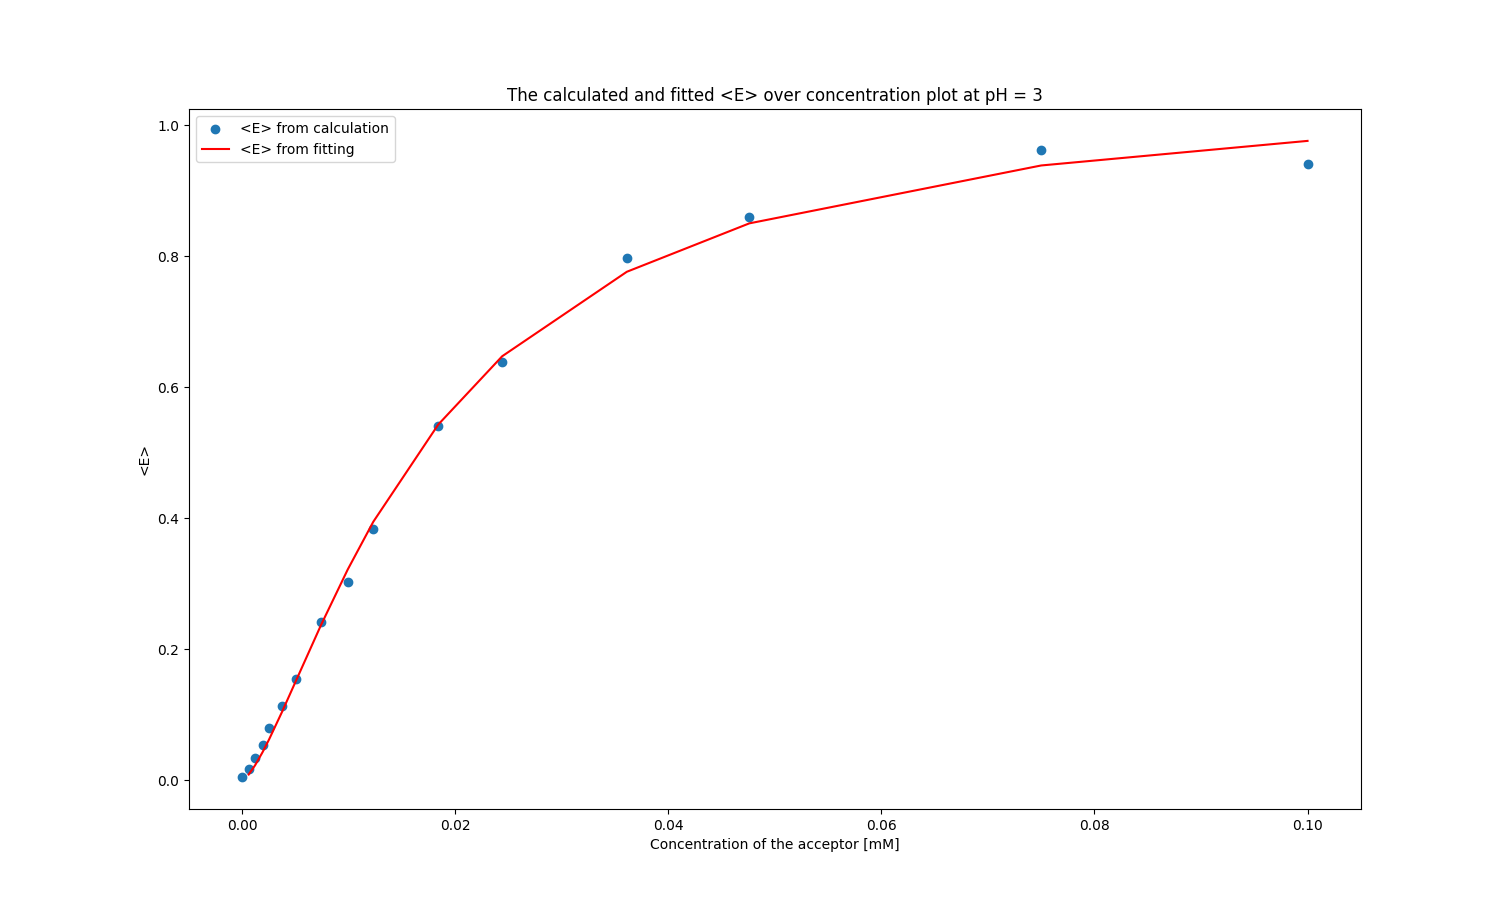
\includegraphics[width=\textwidth]{Figures/E_mean_ph3.png}
        \caption{The real <E>/[A] plot}
    \end{subfigure}
    \quad % Adjust spacing between subfigures as needed
    \begin{subfigure}[b]{0.45\textwidth}
        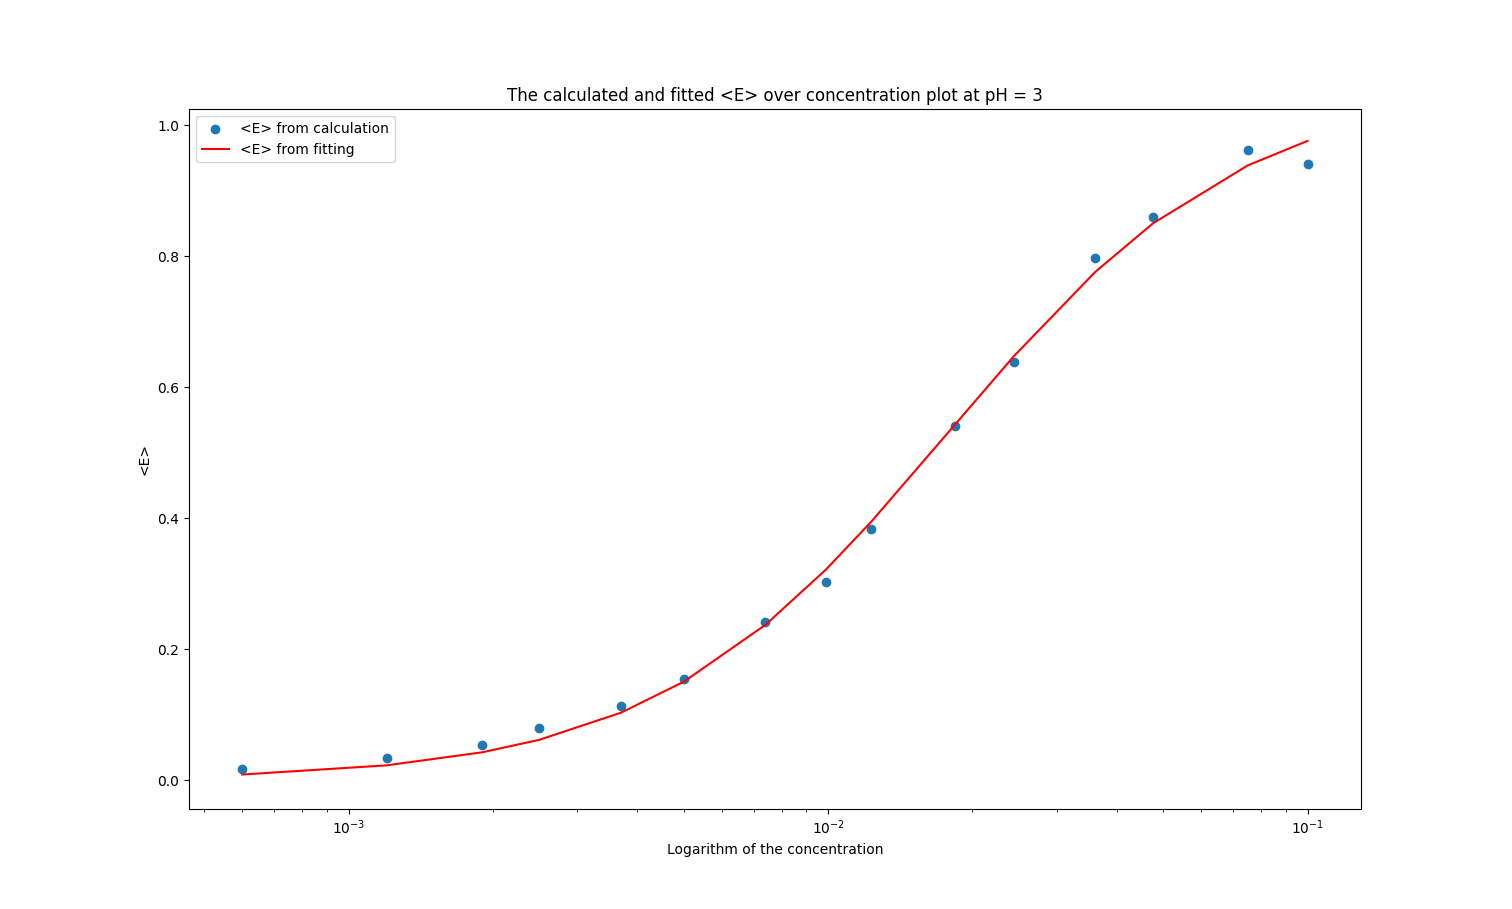
\includegraphics[width=\textwidth]{Figures/Log_e_mean_ph3.png}
        \caption{<E> over logarithm [A]}
    \end{subfigure}
    \caption{<E> over acceptor concentrations under pH3, the blue dots are calculated by the intensity ratio, while the red curve is the 3 parameter fitting result}
\end{figure}


\begin{figure}[htbp]
    \centering
    \begin{subfigure}[b]{0.45\textwidth}
        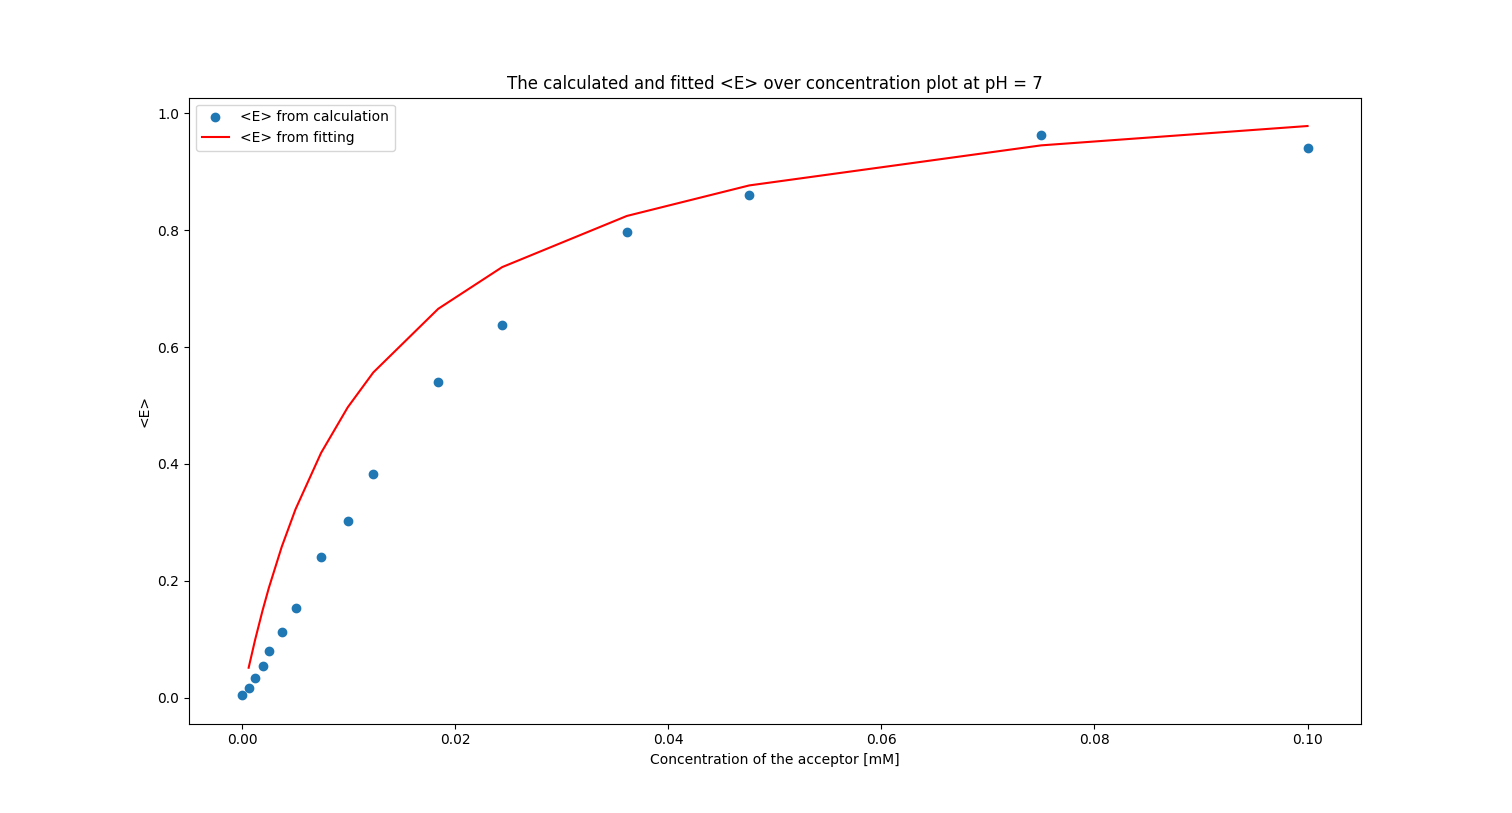
\includegraphics[width=\textwidth]{Figures/E_mean_ph7.png}
        \caption{The real <E>/[A] plot}
    \end{subfigure}
    \quad % Adjust spacing between subfigures as needed
    \begin{subfigure}[b]{0.45\textwidth}
        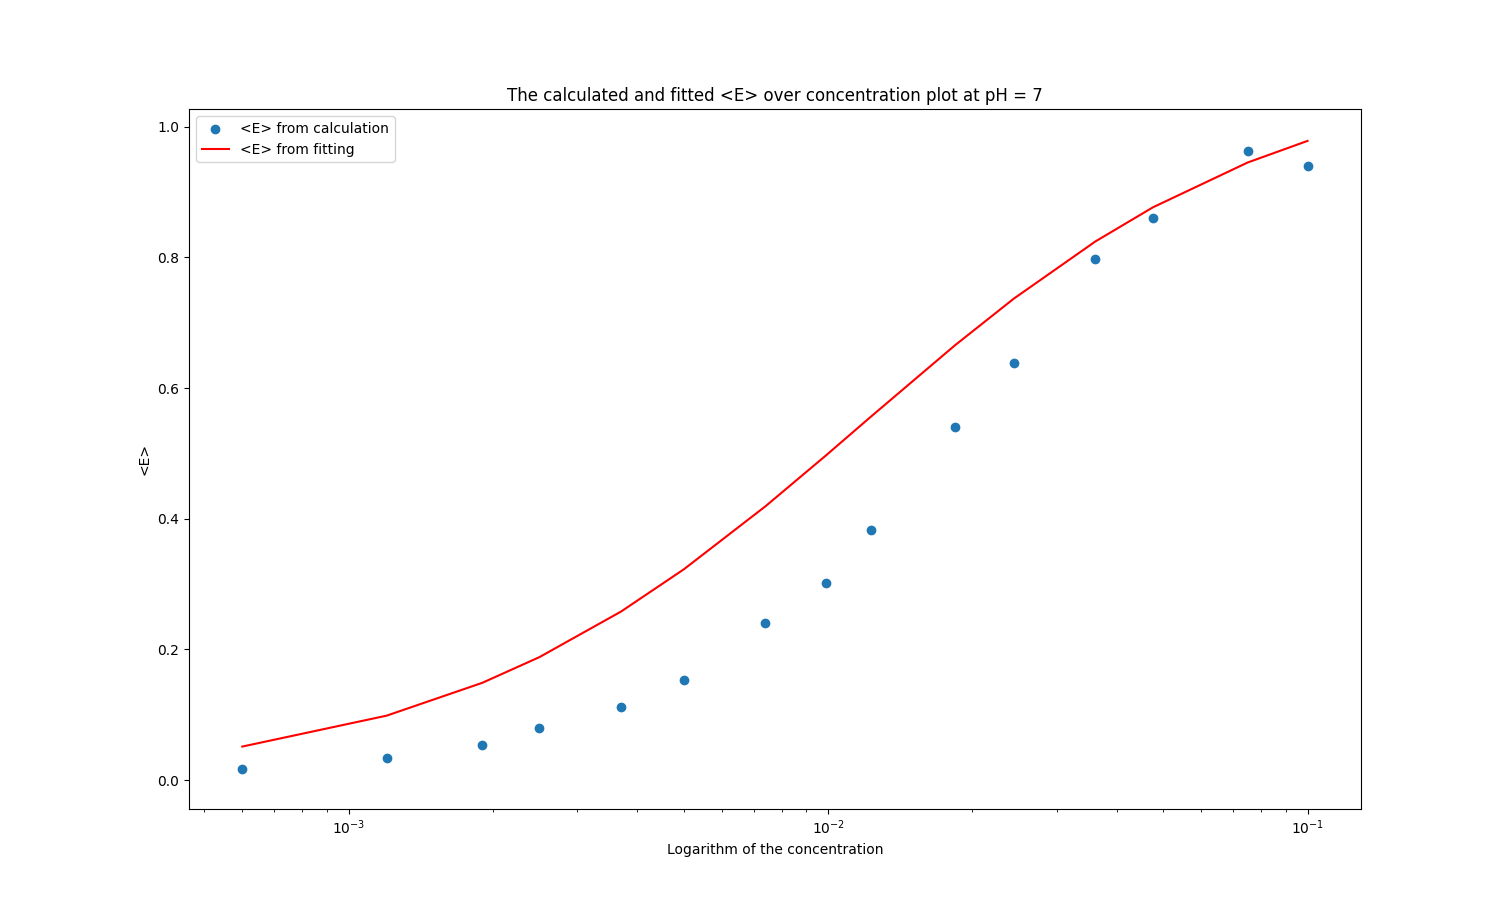
\includegraphics[width=\textwidth]{Figures/Log_e_mean_ph7.png}
        \caption{<E> over logarithm [A]}
    \end{subfigure}
    \caption{<E> over acceptor concentrations under pH7, the blue dots are calculated by the intensity ratio, while the red curve is the 3 parameter fitting result}
\end{figure}
% 3) Stern-Volmer plot, which could determine the K_sv
% 4) concentration over E_mean by <E> = I_d/gamma*I_d+I_a, and fitting with another formula to determine E_max, n and K_D. We can compare K_D and K_SV to see the quenching type (In static quenching, K_D = 1/K_sv)
% 5) Compute the R_0 of the FRET, and compute the effective distance. R_eff = R_0((1-E_max)/E_max)^(1/6)
Finally, we calculated the Föster radius of the HSA and 3-HF FRET pair. By comparing the overlap of the absorption spectra of the acceptor and the emission spectra of the donor (Figure 4.7), we could observe the large area of the spectrum overlap, which makes it reasonable to use the approximation. According to the methods part, we could acquire the following result (Table 4.2):
\begin{table}[hbpt] %9565.217391304348 9942.028985507246
    \centering
    \begin{tabular}{c|c|c|c|c}
        \hline
         pH& $\epsilon$[1/M $\cdot$ cm] &$\lambda$[nm]&J[$m^3/M$]&$R_0$[nm]\\
         \hline
         3& 9565.217 & 330 & 1.134 $\times 10^{-29}$&2.40
         7& 9942.028 & 342 & 1.376 $\times 10^{-29}$&2.48
    \end{tabular}
    \caption{The calculation of the Föster radius}
    \label{tab:my_label}
\end{table}

\begin{figure}[htbp]
    \centering
    \begin{subfigure}[b]{0.45\textwidth}
        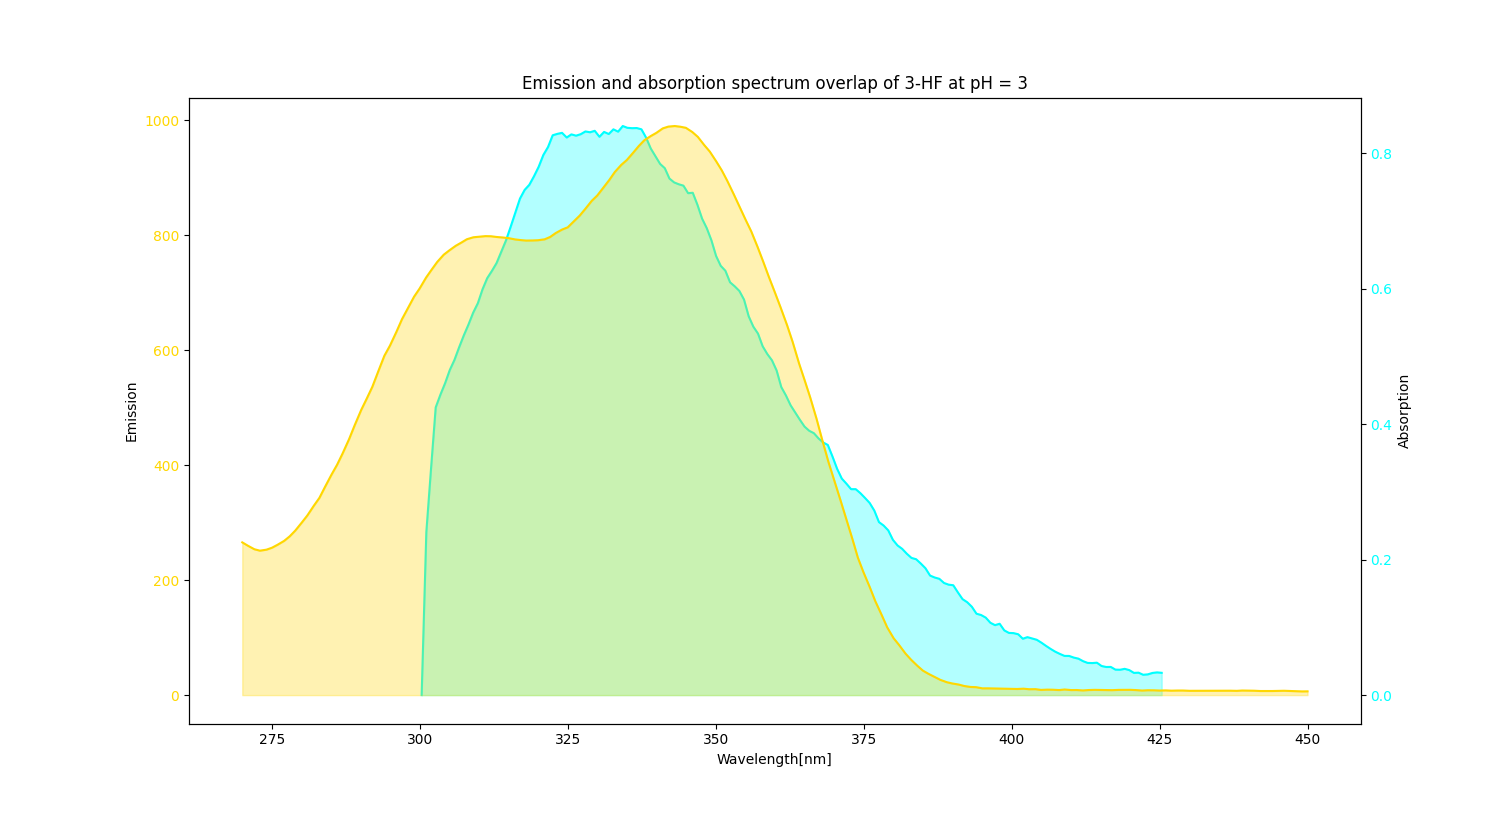
\includegraphics[width=\textwidth]{Figures/spectrum_overlap_ph3.png}
        \caption{pH3}
    \end{subfigure}
    \quad % Adjust spacing between subfigures as needed
    \begin{subfigure}[b]{0.45\textwidth}
        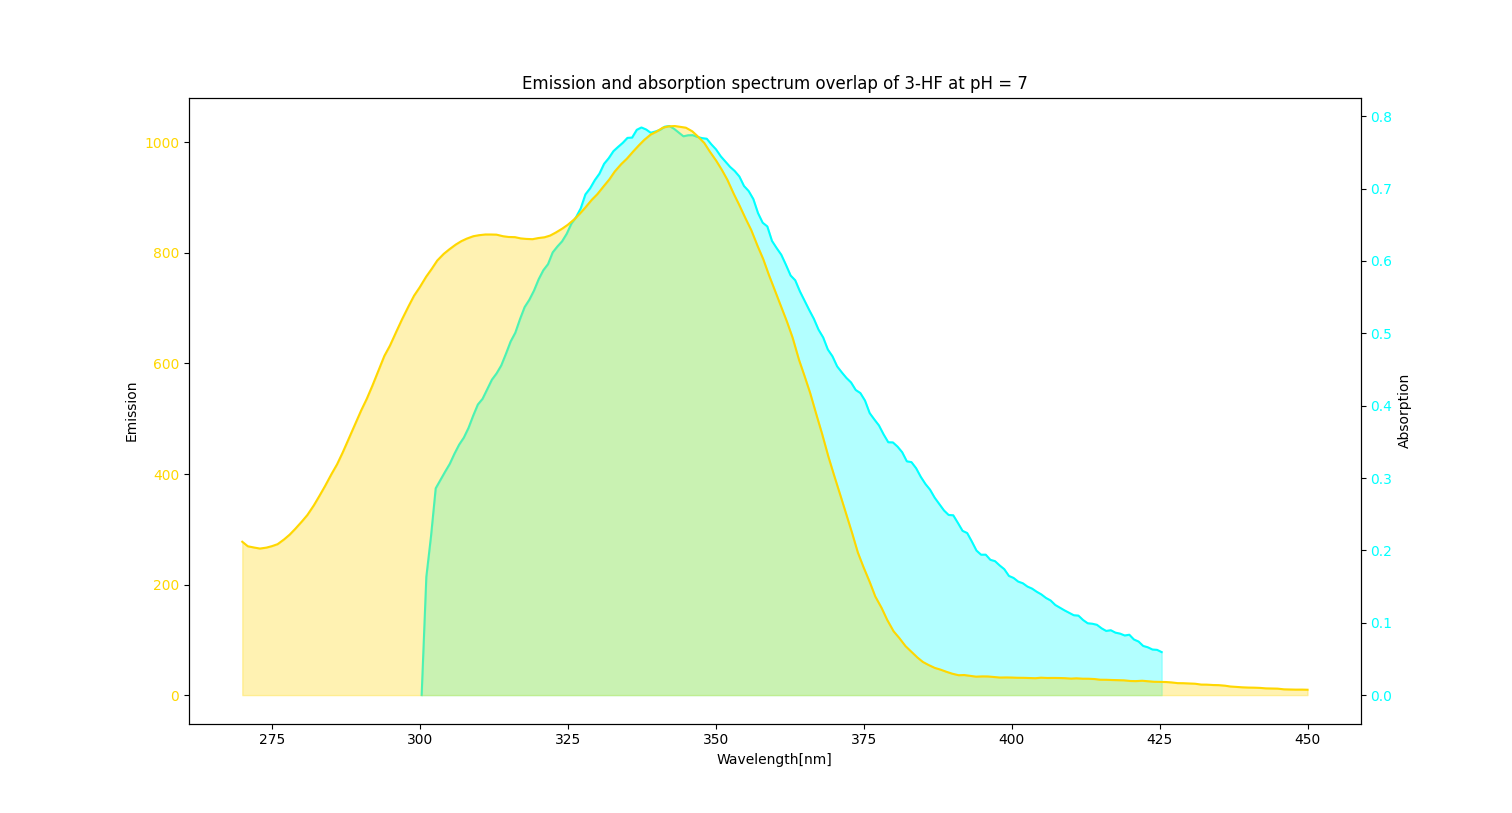
\includegraphics[width=\textwidth]{Figures/spectrum_overlap_ph7.png}
        \caption{pH7}
    \end{subfigure}
    \caption{The emission spectrum of donor and the absorption spectrum of the acceptor}
\end{figure}
\chapter{Discussion}
\label{cha:Discussion}
The following Chapter will discuss the previous results and a general overview of the experiment as a whole.
% 1) The pH influence to the experiment.
The experiment showed that pH significantly impacts the binding interactions and fluorescence behavior of HSA and 3-HF. We also noted that At pH3, the absorption spectra decreased, this could be the result of a lower concentration of protein or of a fraction of the protein being in an unfolded state.  Binding curves further supported pH's role, with KDKD values indicating stronger complex formation at neutral pH, consistent with HSA's physiological role. These findings highlight the importance of considering pH as a crucial factor in FRET experiments involving proteins.\\

% 2) The real quenching type could be mixing type instead of single, which could bring some system errors.
The Stern-Volmer plots and fluorescence data suggest a mixed quenching mechanism rather than purely static or dynamic quenching. Our data also indicated this assumption. By comparing the $\frac{1}{K_D}$(555.55/mM and 833.33/mM) with the $K_{SV}$, we could notice there are large mismatch, saying that our system is not purely static quenching. Static quenching forms non-fluorescent complexes, while dynamic quenching involves collisional interactions.  This mixed quenching introduces systematic errors, complicating FRET efficiency and binding dynamics interpretation. Recognizing and accounting for mixed quenching is essential for accurately analyzing FRET data and understanding the molecular interactions involved. Future experiments should aim to distinguish and quantify these quenching mechanisms to improve data reliability.


\printbibliography
\end{document}